\documentclass[12pt,a4paper,oneside]{article}

\usepackage[utf8]{inputenc}
\usepackage[portuguese]{babel}
\usepackage[T1]{fontenc}
\usepackage{amsmath}
\usepackage{amsfonts}
\usepackage{amssymb}
\usepackage{graphicx}
\usepackage[hyphens]{url}
\usepackage{hyperref}

\author{\\Universidade Federal de Goiás - UFG (Regional Jataí) \\Bacharelado em Ciência da Computação \\Inteligência Artificial \\Prof. Esdras Lins Bispo Jr.}

\title{
	{\sc \huge Lista de Exercícios 2} 
	\\{\tt Versão 1.0}
}

\begin{document}

\maketitle

\begin{enumerate}

	\item Leitura dos capítulos 3 e 4 do Livro {\it Inteligência Artificial} (Russel e Norvig, 2004).
	
	\item Leitura do capítulo 1 do Livro {\it Information Retrieval} (Manning, 2009). Você pode acessar através deste link: \url{https://nlp.stanford.edu/IR-book/pdf/01bool.pdf}.
	
	\item Considerando o seguinte mapa:
	
	\begin{center}
		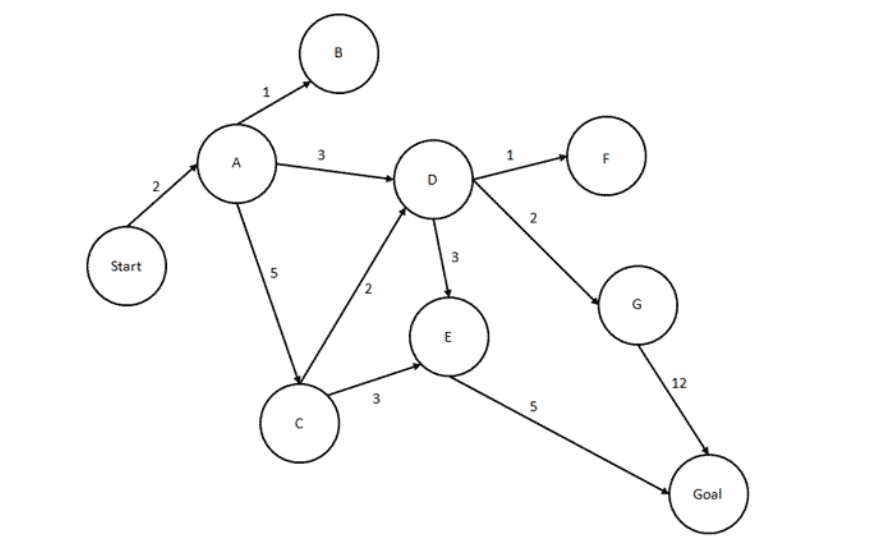
\includegraphics[width=10cm]{images/fig04.png}
	\end{center}
	
	Responda as questões abaixo considerando ``Start'' como o estado inicial e ``Goal'' o estado final buscado.
	
	\begin{enumerate}
		\item Monte as árvores de busca que seriam geradas pelos algoritmos de busca cega vistos em aula (busca em largura, busca de custo uniforme, busca em profundidade, busca com aprofundamento iterativo, busca bidirecional).
		\item Qual dos algoritmos apresentou melhor resultado? Considerando o custo do caminho e o número de nós avaliados até que a solução fosse encontrada.
	\end{enumerate}

	\item Dada a coleção de documentos abaixo:
	
	\begin{itemize}
		\item[] {\bf Doc1} \ \ new home sales top forecasts
		\item[] {\bf Doc2} \ \ home sales rise in july
		\item[] {\bf Doc3} \ \ increase in home sales in july
		\item[] {\bf Doc4} \ \ july new home sales rise
	\end{itemize}
	
	\begin{enumerate}
		\item Construa o índice invertido (conforme apresentado em sala de aula);
		\item Aponte o resultado das consultas:
		\begin{enumerate}
			\item {\tt july} {\sc AND} {\tt sales}
			\item {\tt home} {\sc AND} {\sc NOT} ({\tt in} {\sc OR} {\tt new})
		\end{enumerate}				 
	\end{enumerate}
	
	\item Escreva o pseudocódigo para os operadores do modelo de recuperação de informação booleano:
	\begin{enumerate}
		\item {\sc AND}($termo1$, $termo2$)
		\item {\sc OR}($termo1$, $termo2$)
		\item {\sc XOR}($termo1$, $termo2$)
		\item {\sc NOT}($termo$)
	\end{enumerate}
	
	\item Para as consultas abaixo, podemos realizá-las em tempo $O( x + y )$, em que $x$ e $y$ são os tamanhos da lista de {\it posting}s para {\tt Brutus} e {\tt Caesar}? Se não, qual o melhor tempo possível?
	\begin{enumerate}
		\item {\tt Brutus} {\sc AND NOT} {\tt Caesar}
		\item {\tt Brutus} {\sc OR NOT} {\tt Caesar}
	\end{enumerate}
	
	\item Realize a busca A* e a busca gulosa para encontrar o melhor caminho para chegar a {\tt Bucharest} partindo de {\tt Lugoj}. Construa a árvore de busca criada pela execução do algoritmo apresentando os valores de $f(n)$, $g(n)$ e $h(n)$ para cada nó. Utilize a heurística de distância em linha reta (conforme tabela dada).
	
	\begin{center}
		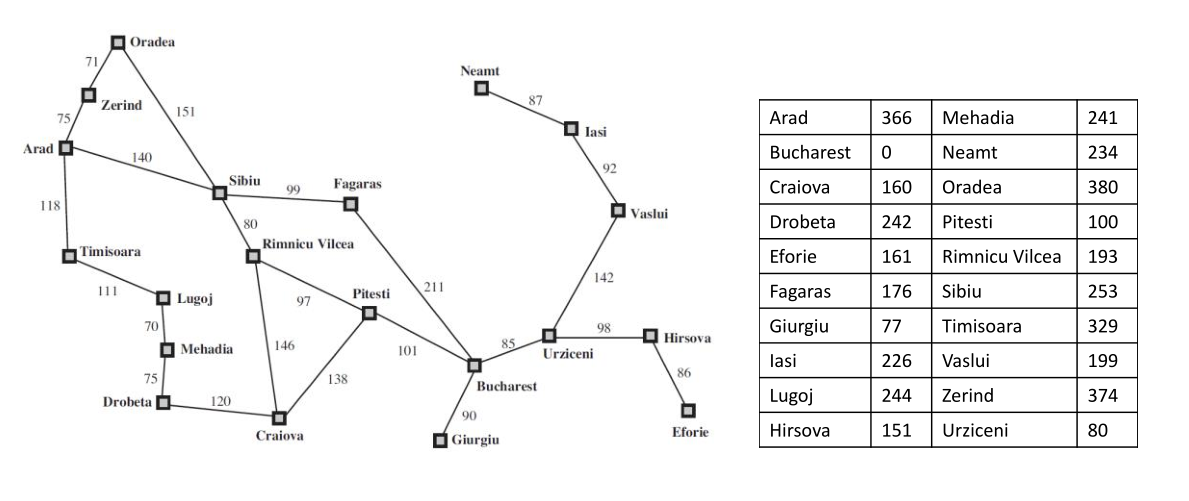
\includegraphics[width=12cm]{images/fig01.png}
	\end{center}
	
	\item O grafo abaixo mostra a ligação entre 5 cidades e as respectivas distâncias em quilômetros:
	
	\begin{center}
		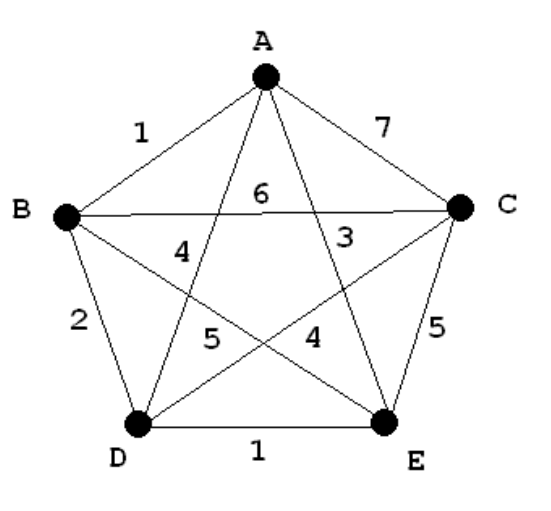
\includegraphics[width=5cm]{images/fig02.png}
	\end{center}
	
	Tem-se um problema em que é necessário passar por todas as cidades, apenas uma vez. O objetivo é encontrar uma rota de menor custo usando um algoritmo genético.
	
	\begin{enumerate}
		\item Proponha uma maneira de codificar os cromossomos.
		\item Defina uma função de aptidão para avaliar a qualidade dos cromossomos.
		\item Gere dois cromossomos e avalie a aptidão deles.
		\item Realize o cruzamento entre os cromossomos.
		\item Aplique uma mutação em um gene dos cromossomos.
		\item Aplique a função de aptidão nos descendentes gerados verificando se a solução encontrada é melhor ou não.
	\end{enumerate}
	
	\newpage
	
	\item Considere a seguinte equação:
	\begin{center}
		$5x + y^2 + w + z^3 = 185$
	\end{center}
	\begin{enumerate}
		\item Proponha uma maneira de codificar os cromossomos.
		\item Defina uma função de aptidão para avaliar a qualidade dos cromossomos.
		\item Defina como o método de seleção dos pais será utilizado.
		\item Defina os operadores genéticos de recombinação e mutação.
		\item Gere uma população inicial de 4 cromossomos e avalie a aptidão deles.
		\item Aplique os operadores de recombinação e mutação sobre essa população para gerar uma nova geração, em seguida avalie a aptidão da nova geração. Repita esse processo por 8 gerações ou até que a solução do problema seja encontrada.
	\end{enumerate}
		
\end{enumerate}

\section{Referências}

\begin{itemize}
	\item RUSSELL, S.; NORVIG, P. {\bf Inteligência Artificial}. Rio de Janeiro: Editora Campus, 2013.
	\item MANNING, C. D,; RAGHAVAN, P,; SCHÜTZE, H. {\bf Introduction to Information Retrieval}, Cambridge University Press. 2008.
\end{itemize}

\end{document}